\section{Selektion}\label{selection}

% http://www.geatbx.com/docu/options-02.html

\subsection{Stochastic Universal Sampling (selsus)}
Die Individuen werden so auf
den Gesamtbereich abgebildet, dass jedes Individuum einen Bereich erhält, dessen
Größe mit der Güte des Individuums korrespondiert, wobei die Individuen mit den
besten Bewertungen die größten Bereiche erhalten und somit auch die höchste
Wahrscheinlichkeit besitzen, gezogen zu werden.

Beim Ziehen werden die Zeiger gleichmäßig über den Gesamtbereich verteilt, was
die Güte des Ziehens verbessert. Wenn N Individuen gezogen werden sollen, ist
der Abstand zwischen den einzelnen Zeigern 1/N und die Position des ersten
Zeigers wird zufällig im Bereich [0, 1/N] bestimmt, wie in Abbildung
\ref{fig.selection}a dargestellt ist.

\begin{figure}[!h] \centering
    \subfigure[Stochastic Universal Sampling]{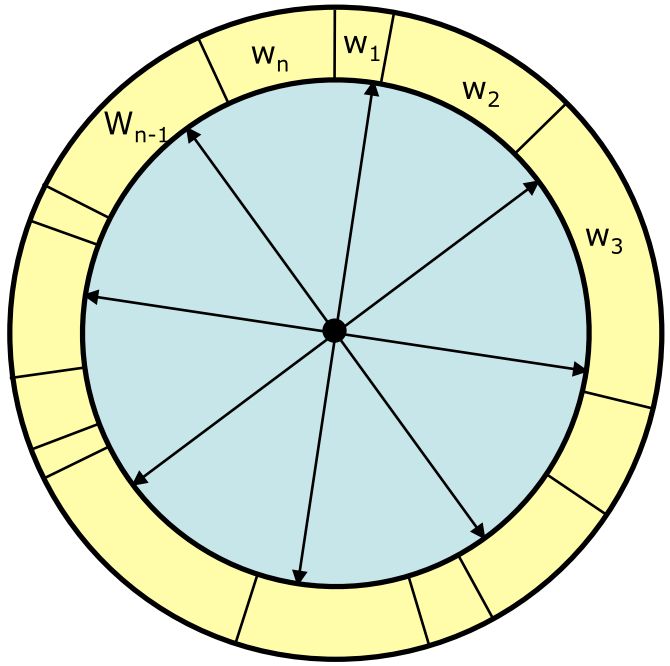
\includegraphics[width=0.49\textwidth]{Figures/selsus.png}}\hfill
    \subfigure[Roulette Wheel Selection]{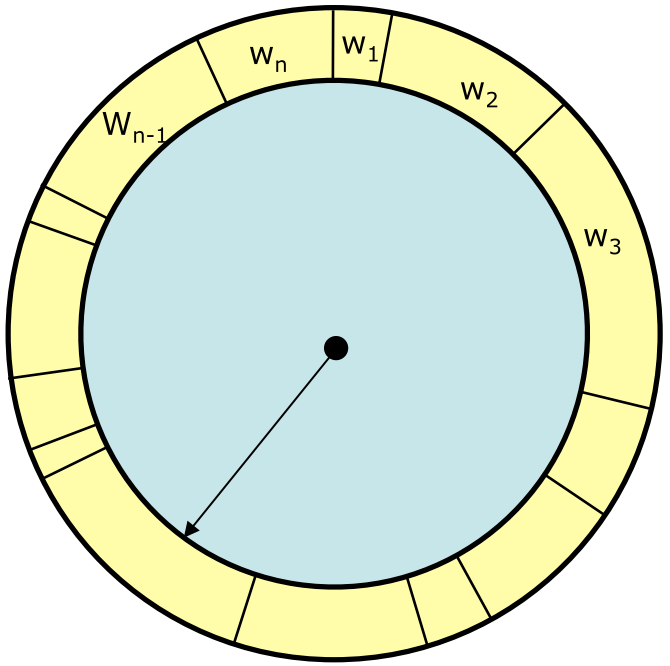
\includegraphics[width=0.49\textwidth]{Figures/selrws.png}}
    \caption{Selektions-Verfahren \citep{mcl}}
    \label{fig.selection}
\end{figure}


\subsection{Tournament Selection (seltour)}
Die Tournament Selection ist ein weiteres Selektionsverfahren,
welches von \emph{GEATbx} zur Verfügung gestellt wird. Das zugrundeliegende
Prinzip ist relativ einfach, eine gewisse Anzahl von Individuen wird zufällig
aus der Population ausgewählt, wobei die Größe dieser Gruppe als \emph{Tour}
bezeichnet wird. Aus dieser Gruppe wird nun das beste Individuum ausgewählt und
zu der Selektion hinzugefügt. Diese 2 Schritte werden so häufig wiederholt, bis
die gewünschte Anzahl an Individuen selektiert ist \citep{seltour}.


\subsection{Ergebnisse}
Die beiden oben genannten Verfahren werden gegenüber dem
klassischen \emph{Roulette Wheel Selection} (selrws) getestet, welches alle
Individuen einzeln per Zufall aus der Population auswählt (siehe Abbildung
\ref{fig.selection}b), dabei kann natürlich
auch ein Genom mit geringer Wahrscheinlichkeit mehrfach ausgewählt werden.

\input{Chapters/gen/Selection.Name}

\begin{figure}[h!]
  \centering
  \includegraphics[width=1.0\textwidth]{Figures/gen/Selection.Name.png}
  \caption{Selektions-Verfahren}\label{fig.selectionname}
\end{figure}

\noindent Die verschiedenen Resultate sind in Tabelle \ref{Selection.Name}
dargestellt. Das \emph{Tournament Selection}-Verfahren schneidet mit deutlichem
Abstand am besten ab (siehe Abbildung \ref{fig.selectionname}) und wird deswegen
auch für die endgültige Konfiguration ausgewählt.

